The preprocessing module receives the message with the structure given by the extraction module and modifies the e-mail so that it can be interpreted by the spaCy's pretrained model. As it is shown in Figure \ref{fig:umlprep}, this UML package has three different UML classes: \textit{PreprocessorApp}, \textit{Preprocessor} and \textit{PreprocessedMessage}.

\begin{figure}[p]
	\centering%
	\centerline{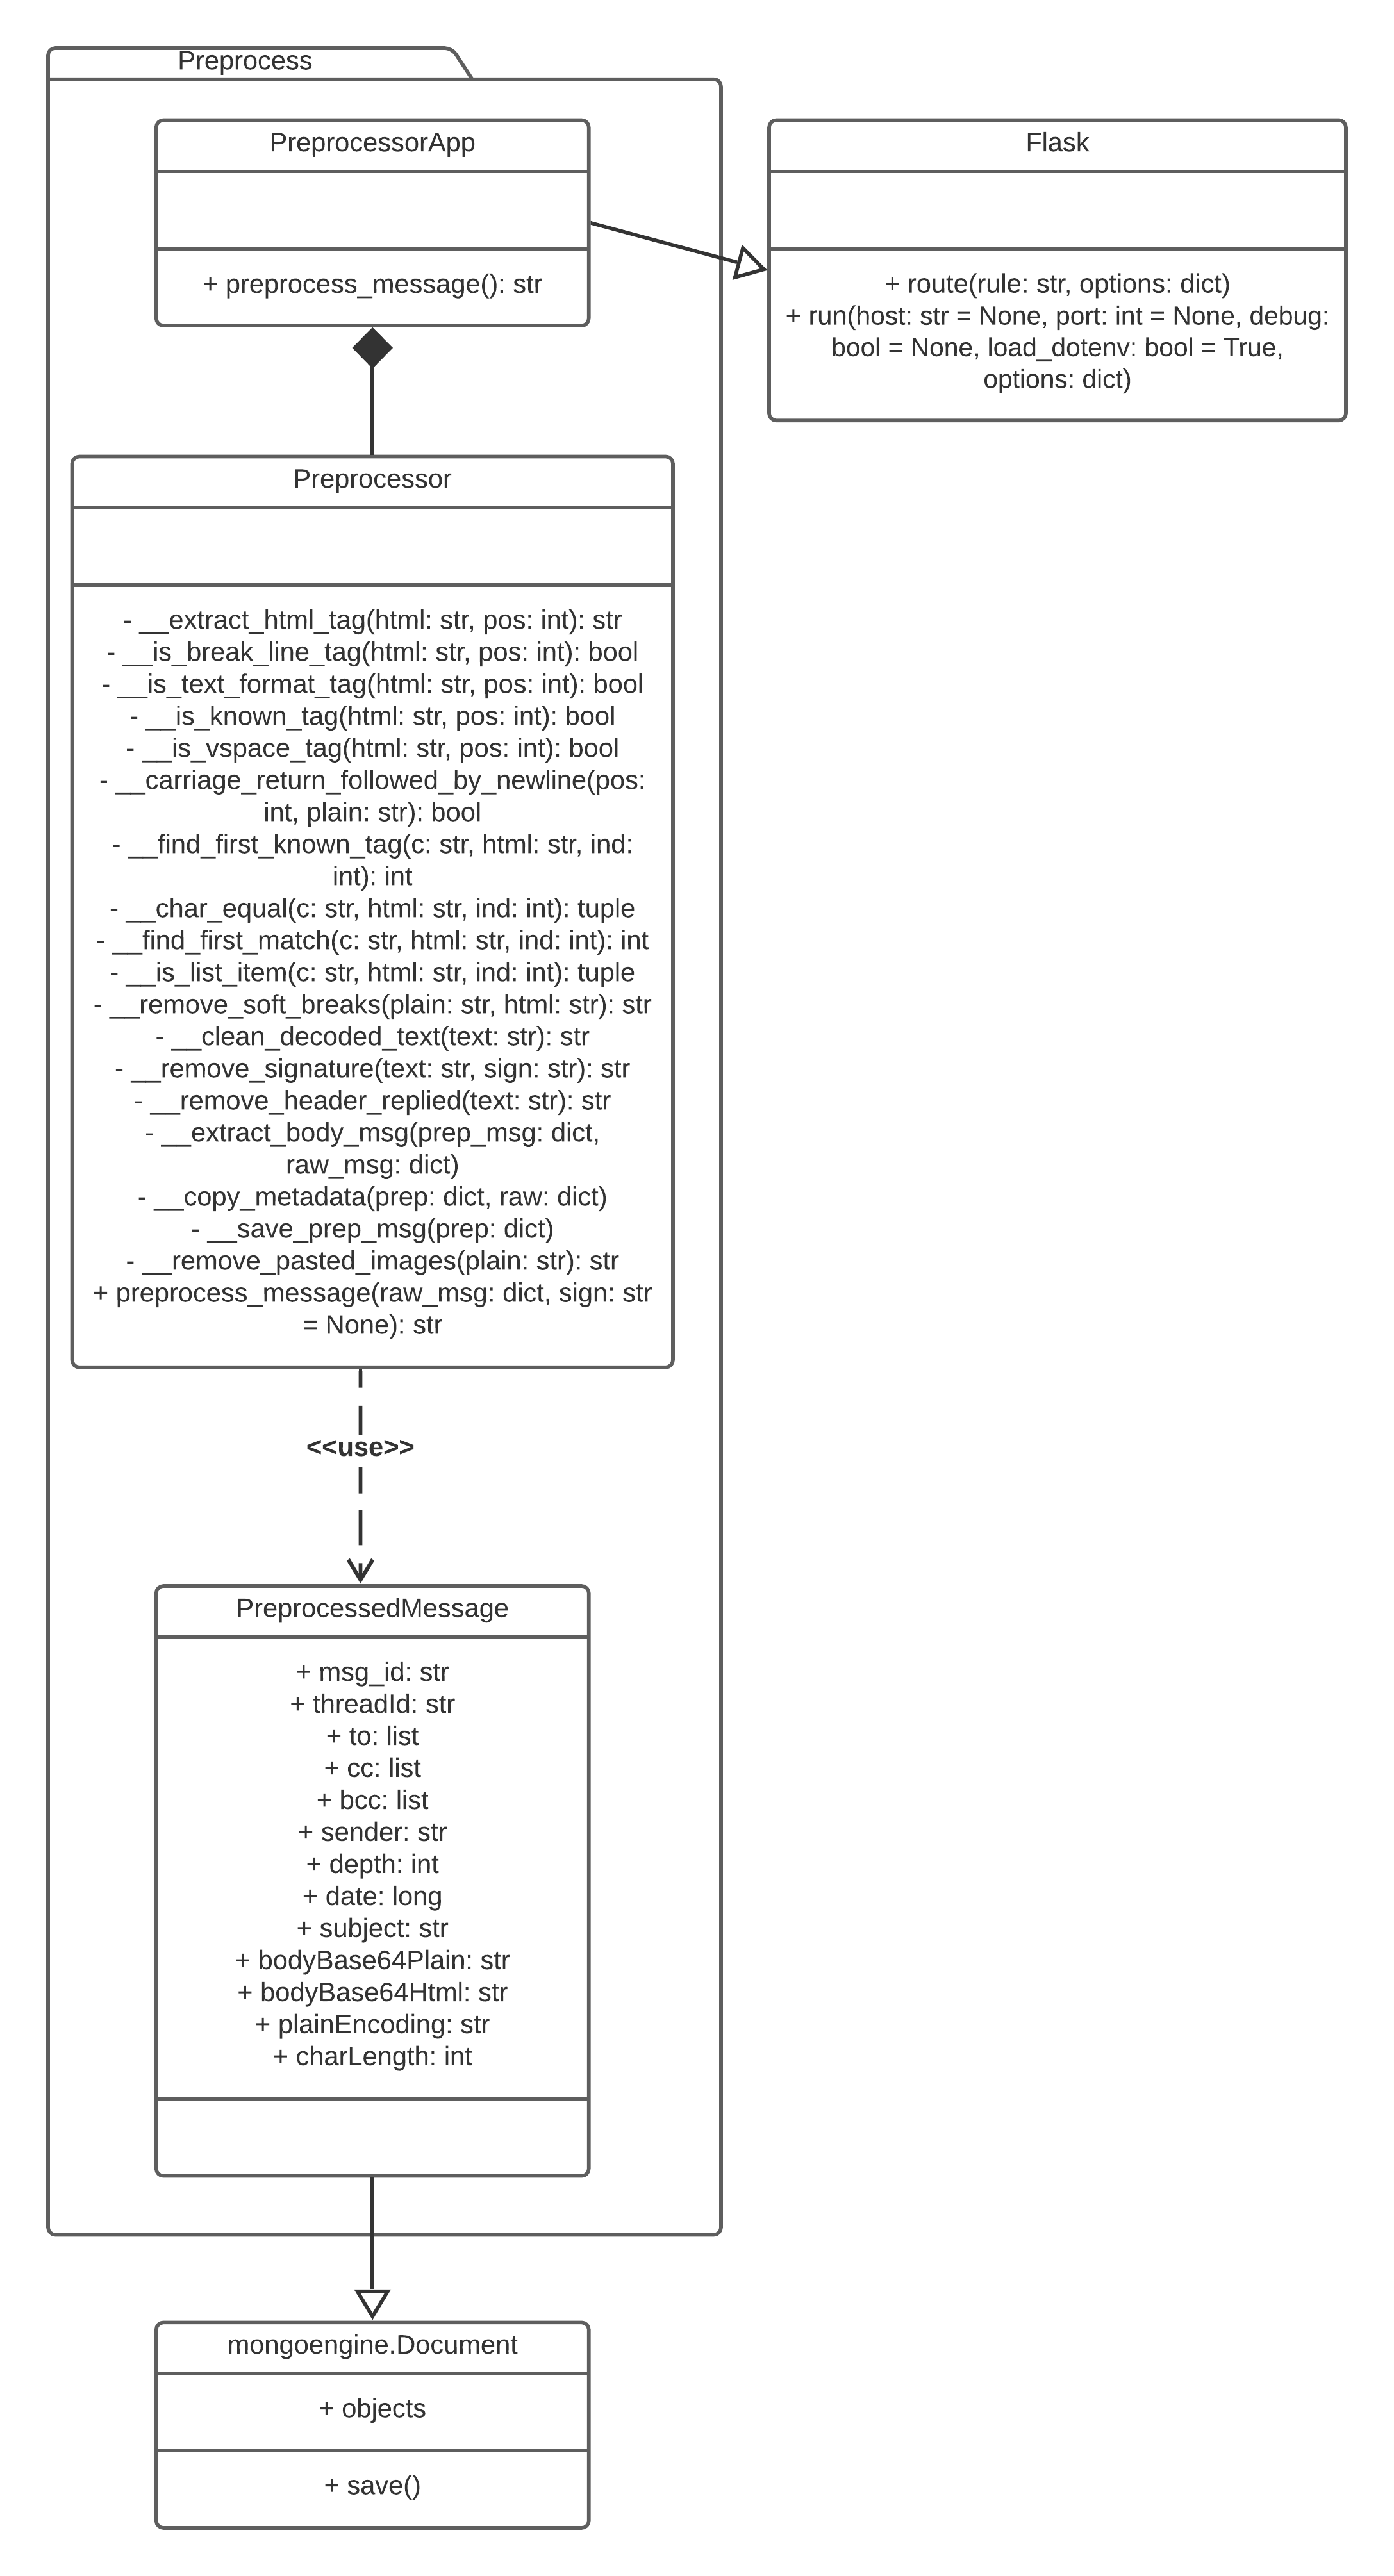
\includegraphics[height=0.8\paperheight]{Imagenes/Bitmap/Analyser/preprocessUML.png}}%
	\caption{UML class diagram of the preprocessing module}%
	\label{fig:umlprep}
\end{figure}

First of all, we can observe the \textit{PreprocessorApp} class. It inherits from \textit{Flask} class (see Section \ref{sect:flask}), which implements a simple web service. Consequently, if we want to preprocess a message, it will be necessary to execute a POST HTTP request with the e-mail as a \textit{json} in it. Having done so, the \textit{preprocess\_message} method will be invoked and send the given message structure to the \textit{Preprocessor} class by calling its only public method: \textit{preprocess\_message}. There is also the possibility of transmitting the user's e-mail signature to the \textit{Preprocessor} (so that it can be removed from the different messages) by including it as an string in the sent \textit{json}.

The main class of this UML package is the \textit{Preprocessor} class. It is in charge of modifying the given message. For this reason, it has different methods which implements the distinct tasks that it has to carry out.

The first task this module performs is to filter those e-mails whose message body as plain text is empty, which means that they lack the \textit{bodyBase64Plain} field. As our purpose is analyse the writing style of the user, we are not interested in e-mails without text. Thus, these messages are discarded.

Then, the images inserted in the message body (not as an attachment) are removed by calling the \textit{\_\_removed\_pasted\_images} method. This function make use of the simple Python's regular expression \pythoninline{r'\\[image:[\^\\]]+\\]'}, detects the position of the different images with it and takes them away.

Once pasted images are removed, the \textit{\_\_extract\_body\_msg} method removes the text of replied e-mail (if it exists) and the soft break lines inserted in the body, as a consequence of the established format in \cite{rfc2646}. When someone replies an e-mail from a Gmail account, the replied message is automatically included under the response (indeed it is possible to intersperse the answer and the responded text). As it is not a written composed by our user, this copied text must be taken away. To this end, the \textit{Preprocessor} class creates an object of the \textit{EmailReplyParser} class of the \textit{email\_reply\_parser}\footnote{\url{https://pypi.org/project/email_reply_parser/0.1.0/}} Python's library. With its \textit{parse\_reply} method, only the response is obtained with the replied message's header automatically included (\textit{EmailReplyParser} class does not remove it). However, such header is easy to detect by using regular expressions, due to it has an specific format as the following line (written in Spanish):

\textit{El mié., 27 may. 2020 a las 11:11, Name (<example@mailserver.com>) escribió:}

The designed regular expression detects this type of sentences with the moment (date and time) and the sender. Once \textit{Preprocessor} knows its position, it is possible to take it away.

A similar problem appears with forwarded messages. Nevertheless, unlike replied e-mails, it is not possible to detect if the user has interspersed new text in the forwarded written. For this reason, \textit{Preprocessor} detects the forwarded header, which indicates the beginning of the resent message, and deletes all the text from it.

In addition to the replied or forwarded text, we find the problem of the inserted soft break lines in order to follow the standard format for sending e-mails. We have implemented two solutions for this issue in \textit{\_\_clean\_decoded\_text} and \textit{\_\_remove\_soft\_breaks} methods. The first function deletes all soft break lines in messages encoded with quoted-printable (see Section \ref{sssect:quot-p}). The second, compares the message body as HTML text and as plain text and removes all soft break lines that do not appear as an HTML tag. Moreover, during this process we detects characters that should not appear in the plain text. For instance, Gmail delimits the text in bold with the symbol ``*'' (there are more examples as the beginning of a bulleted list, an enumeration or the change of font or font size). As in the HTML text it will appear between two tags, we recognise this fact and take the delimiter character away. In this way we are able to obtain a real plain text.

The last modification made by the preprocessor is the removal of the signature. This only happens if the user has provided it to the system, since the recognition of the signature is a complex problem that is not the objective of this work. The \textit{\_\_remove\_signature} method is is responsible for carrying out that task.

Once an extracted e-mail is preprocessed, it is ready to be saved in the database. As it happened with the \textit{ExtractedMessage} class, the \textit{PreprocessedMessage} class inherits from the \textit{mongoengine.Document} class, allowing it to insert elements in the database. If we compare the \textit{ExtractedMessage} and \textit{PreprocessedMessage} class, we will realise that they have the same attributes, so a preprocessed message has the same structure as an extracted one.